\documentclass[letterpaper,10pt]{article}

\usepackage{enumitem}
\usepackage{titling}
\usepackage{listings}
\usepackage{url}
\usepackage{hyperref}
\usepackage{setspace}
\usepackage{subfig}
\usepackage{sectsty}
\usepackage{pdfpages}
\usepackage{colortbl}
\usepackage{multirow}
\usepackage{multicol}
\usepackage{relsize}
\usepackage{amsmath}
\usepackage{wasysym}
\usepackage{fancyvrb}
\usepackage[yyyymmdd]{datetime}
\usepackage{amsmath,amssymb,amsthm,graphicx,xspace}
\usepackage[titlenotnumbered,noend,noline]{algorithm2e}
\usepackage[compact]{titlesec}
\usepackage{XCharter}
\usepackage[T1]{fontenc}
\usepackage[scaled]{beramono}
\usepackage[normalem]{ulem}
\usepackage{booktabs}
\usepackage{tikz}
\usetikzlibrary{arrows,automata,shapes,trees,matrix,chains,scopes,positioning,calc}
\tikzstyle{block} = [rectangle, draw, fill=blue!20,
text width=2.5em, text centered, rounded corners, minimum height=2em]
\tikzstyle{bw} = [rectangle, draw, fill=blue!20,
text width=4em, text centered, rounded corners, minimum height=2em]

\definecolor{namerow}{cmyk}{.40,.40,.40,.40}
\definecolor{namecol}{cmyk}{.40,.40,.40,.40}
\renewcommand{\dateseparator}{-}

\let\LaTeXtitle\title
\renewcommand{\title}[1]{\LaTeXtitle{\textsf{#1}}}

\lstset{basicstyle=\footnotesize\ttfamily,breaklines=true}

\newcommand{\handout}[5]{
	\noindent
	\begin{center}
		\framebox{
			\vbox{
				\hbox to 5.78in { {\bf ECE 252: Systems Programming and Concurrency } \hfill #2 }
				\vspace{4mm}
				\hbox to 5.78in { {\Large \hfill #4  \hfill} }
				\vspace{2mm}
				\hbox to 5.78in { {\em #3 \hfill \today} }
			}
		}
	\end{center}
	\vspace*{4mm}
}

\newcommand{\lecture}[3]{\handout{#1}{#2}{#3}{Lecture#1}}
\newcommand{\tuple}[1]{\ensuremath{\left\langle #1 \right\rangle}\xspace}

\newcommand{\Rplus}{\protect\hspace{-.1em}\protect\raisebox{.35ex}{\smaller{\smaller\textbf{+}}}}
\newcommand{\Cpp}{\mbox{C\Rplus\Rplus}\xspace}


\addtolength{\oddsidemargin}{-1.000in}
\addtolength{\evensidemargin}{-0.500in}
\addtolength{\textwidth}{2.0in}
\addtolength{\topmargin}{-1.000in}
\addtolength{\textheight}{1.75in}
\addtolength{\parskip}{\baselineskip}
\setlength{\parindent}{0in}
\renewcommand{\baselinestretch}{1.5}
\newcommand{\term}{Spring 2019}
\newcommand{\termnumeric}{1195}

\singlespace


\begin{document}

\lecture{ 7 --- Sockets }{\term}{Jeff Zarnett}

\section*{Network Communication}

Another form of inter-process communication is of course the idea of network communication. If two processes are not running on the same machine in the same environment, then to get them to communicate we can't use pipes or shared memory... instead, we must communicate over the network. But not only that: we can actually use the network as a method of communication if the two processes are on the same machine (as we will see).

A diagram describing network communication frequently represents the network as just a mysterious cloud or blob, and for the moment we will just pretend that is how it is. There is a whole course on how computer networks function and behave and what the various layers are. For the sake of simplicity we will focus just on how we use the network, and not how the network is implemented.

\subsection*{Sockets}

The \textit{socket} API is a standard dating back many years, describing how to communicate over the network in a standard way. The socket is the concept for how to establish a communication channel between two processes. There are really two ways that we can communicate: datagrams and connection streams.

A datagram is a lot like sending a letter in the mail (you know, snail mail): you can mail out letters but they can be delivered in any order, might get lost along the way, and are unidirectional~\cite{apunix}. The recipient of a letter can write one back if desired but it may not be. There's no ``connection'' to be established, it's just message delivery.

The stream is like making a telephone call. When you dial a number, the other side has to be available (i.e., not on the phone or away from their phone) and if they answer then a line of communication is established to allow exchange of data (talking). Then at some point one party or the other will hang up and that's the end of the call. The telephone network has to do quite a bit to get your data from one end to the other in a timely manner, but that's not really your concern at the time that you want to make the phone call.

Much like everything else in UNIX, a socket is handled like a file. It just so happens that when you open a socket, the data to be read or written from the ``file'' is being routed over the network somehow. To create a socket, we need the \texttt{sys/socket.h} header included and the call is~\cite{apunix}:

\begin{lstlisting}[language=C]
int socket( int domain, int type, int protocol )
\end{lstlisting}

The arguments require some explanation. The \texttt{domain} value defines the address format (amongst other things) and is how we would choose between, for example, IPv4 and IPv6 (or other more things...). For the purposes of this course, we'll use IPv4 and the constant for that is defined as \texttt{AF\_INET} (address family: internet!).

The \texttt{type} argument gives what kind of information we are going to be sending. \texttt{SOCK\_DGRAM} is for datagrams and \texttt{SOCK\_STREAM} is for a bidirectional byte stream~\cite{apunix}.

The \texttt{protocol} argument is about how the data is to be transported over the connection, and we will just use 0 for the default. If we chose a stream, the default is TCP/IP. Without going into too much detail, TCP/IP is the way a lot of data is transported over the internet. This is a (generally) reliable method of transport that makes sure your data gets to where it needs to go, with all the pieces in the correct order. If we chose a datagram, the default is UDP, which is not a reliable method of communication: data packets might get there or they might not.

Notice that the return type is an integer. Why is that? Well, a file descriptor is really just an integer, as we already saw with the pipe examples. So as long as we remember that's what the integer represents, we will not have any problems.

And just like a file that is opened, a socket that is opened needs to be closed when we are finished with it. For that we can just use \texttt{close}. You have probably noticed some asymmetry: there are different calls to open things (\texttt{open}, \texttt{pipe}, \texttt{socket}). That's because when we want to open something we have to say what kind of thing we want to open. When we want to close something, we already know what type it is.

\paragraph{Check the Boot of the Car for your Jumper!}
When we are going to communicate over the network we have to make sure that we speak the same language. More than that, we have to speak the same dialect (British English, for example, contains phrases and terms that you might not know if you only know Canadian or American English).

Normally this is not something that we need to think about, but when communicating over the network, the system on the other side might have a different idea of how data is organized. Consider, if you will, a four byte (32 bit) integer. There are two possible (reasonable) orders for how its bytes can be stored: smallest to largest or largest to smallest. These are shown below as big-endian and little-endian respectively:

\begin{center}
	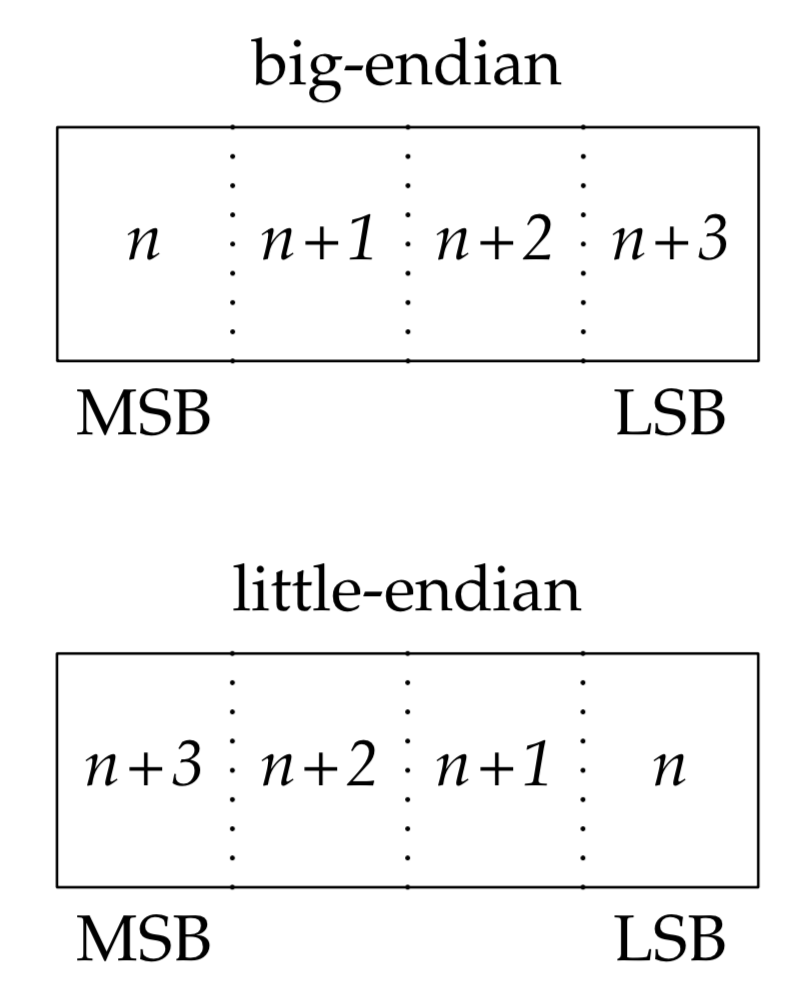
\includegraphics[width=0.25\textwidth]{images/endian}\\
	Byte order for a 4-byte (32 bit) integer~\cite{apunix}.
\end{center}

You might think that little-endian makes no sense. This is because you are a human reading a language left to right in a case where we put lower memory addresses on the left and higher ones on the right. The computer does not care about the convention. But anyway, x86 architecture is little-endian, but others (PowerPC) are not, so we can make no assumptions about what the architecture of the other side is. For this reason, network protocols specify a particular byte ordering so that everyone agrees on the meaning of the material. And this means that we need to translate the values to the big-endian format.

Included in the \texttt{arpa/inet.h} header are some functions to help us out. They translate from whatever system byte order you have to the network byte order, and vice versa. Their use is advisable even if you're sure the system you are using is big-endian, because of portability of your code. They come in 32-bit and 16-bit variants depending on what you need.

\begin{lstlisting}[language=C]
uint32_t htonl( uint32_t hostint32 ) /* Translate 4 byte int to network format */
uint16_t htons( uint16_t hostint16 ) /* Translate 2 byte int to network format */
uint32_t ntohl( uint32_t netint32 )  /* Translate 4 byte int to host format */
uint16_t ntohs( uint16_t netint16 ) /* Translate 2 byte int to host format */
\end{lstlisting}

Wait, these don't look like integers, or unsigned integers, do they? Well, sometimes we want to be very specific about the size of the integer. As you can imagine, this routine doesn't work if you don't know how big of an integer you're dealing with. And sometimes we will need to be specific about sizes.

\paragraph{Addresses.} Right, so keeping this in mind, when we want to call someone, we have to put in their phone number. And if we want someone to call us, we need a phone number and we need to be ready to receive calls. This number has to be translated to the right format, sure, but we're able to do this using those functions above. The structure for a socket address is \texttt{struct sockaddr\_in}. The structure has three fields, and below is a sample initialization~\cite{apunix}:

\begin{lstlisting}[language=C]
struct sockaddr_in {
  sa_family_t sin_family; /* Address family */
  in_port_t sin_port; /* Port number */
  struct in_addr sin_addr; /* IPv4 Address */
};

struct sockaddr_in addr;
addr.sin_family = AF_INET;
addr.sin_port = htons( 2520 );
addr.sin_addr.s_addr = htonl( INADDR_ANY );
\end{lstlisting}

As expected, if we want an IPv4 address then we use the matching family type of \texttt{AF\_INET}. Then there are the IP address and port fields.

You're almost certainly familiar with IPv4 addresses... they take the format of \texttt{XXX.XXX.XXX.XXX} where each grouping of \texttt{XXX} is a number between 0 and 255. If you want to connect to your router, for example, you might type in \texttt{192.168.0.1} in the address bar of your browser. When you type in a name, like \texttt{uwaterloo.ca} there is a translation process that occurs that transforms this into an IP address, like \texttt{129.97.208.23}. The computer uses the number; names are nice for humans, though. But here we chose a constant value, \texttt{INADDR\_ANY}. This says, choose the current IP address of the current computer (and it could have several if it has more than one network connection). We aren't trying to use any specific address; we just want one the computer has.

And what about ports? If you want to think about your computer's address as being like a street address, imagine that it's then an apartment building and the port number is which apartment the connection is made with. Different services (processes) are communicating over different ports. No two processes can be using the same port at the same time. By convention, ports with numbers below 1024 considered to be reserved for system services (and requiring superuser access to make use of). For our purposes, we will always choose ports above 1024.

When you log in to a server with \texttt{ssh}, for example, the default port for that is 22. This is a ``well known'' port, in that everyone agrees up front this port is the one for this service. Thus when a server starts up the daemon, it knows to listen for connections on port 22 and when you're ready to connect to that server, the \texttt{ssh} client chooses that port by default.

\paragraph{Looking Up the Address.}
In real life, we probably only rarely use IP addresses directly when trying to connect to services. If you already know it, that's fine, but more likely you use a human-friendly name. For example, you use \texttt{ssh username@ecelinux.uwaterloo.ca} and don't need to manually look up the IP address for the server. You can, of course (the command line tool is \texttt{nslookup}), but why should you have to? The computer can do this for you.

Looking up hostnames and the like is somewhat complex (and not the focus), so we will just learn one method for doing this. Many examples and older texts use the function \texttt{gethostbyname()}, but this is now deprecated and has been replaced with the \texttt{getaddrinfo()} function instead. You might still see it in the wild but we should learn the new way.

The function is prototyped in in \texttt{netdb.h} and looks like this~\cite{getaddrinfo}:
\begin{lstlisting}[language=C]
int getaddrinfo(const char *node,     // e.g. "www.example.com" or IP
                const char *service,  // e.g. "http" or port number
                const struct addrinfo *hints,
                struct addrinfo **res);
\end{lstlisting}

The \texttt{node} parameter is the hostname to connect to but can also be an IP address. The \texttt{service} parameter can be things like ``http'' to get the defined port for that protocol, but I really recommend you use explicit port number such as ``80'' for HTTP. The \texttt{hints} parameter is used (optionally) to restrict what kind of connection you want, such as saying you want IPv4, TCP Stream sockets, and letting the function fill in the IP address (see example below). And then there is a pointer to a \texttt{struct addrinfo *} (pointer to a pointer); that structure will be updated when the function is done. And the function does have a return value of an int, whereby 0 indicates success.

Okay, so let's try it out~\cite{getaddrinfo}:

\begin{lstlisting}[language=C]
struct addrinfo hints;
struct addrinfo *serverinfo;  // will point to the results

memset(&hints, 0, sizeof hints); // make sure the struct is empty
hints.ai_family = AF_INET;     // Choose IPv4
hints.ai_socktype = SOCK_STREAM; // TCP stream sockets
hints.ai_flags = AI_PASSIVE;     // fill in my IP for me

int result = getaddrinfo("www.example.com", "2520", &hints, &serverinfo);
if (result != 0) {
  return -1;
}
struct sockaddr_in * sain = (struct sockaddr_in*) serverinfo->ai_addr;
/* Do things with this */

freeaddrinfo( serverinfo );
\end{lstlisting}

Assuming that all went well, the \texttt{serverinfo} pointer is now pointing to a linked list of \texttt{struct sockaddr} (the generic form of \texttt{sockaddr\_in}) which gives us the information we need: the IP address for the server we want to communicate with. The actual info struct is in the linked list node's \texttt{ai\_addr} attribute and the pointer to the next one is \texttt{ai\_next}. Most of the time we just need the first result, though. The \texttt{struct sockaddr} structure we got out of this can be used in future calls (although we might need to cast the result to the type we need).

If we are interested in getting the structure for the local computer, we can manually initialize the \texttt{struct sockaddr\_in} as we did before learning about how \texttt{getaddrinfo()} works. Or we can call \texttt{getaddrinfo()} with \texttt{NULL} as the \texttt{node} parameter.

As some further notes, it's possible to use \texttt{NULL} for the hints if you are willing to accept the defaults (we usually are if we're sure about the type of result we will get). To deallocate the information that has been allocated, the call is \texttt{freeaddrinfo()} as shown above.

\paragraph{Client: Connect.}
Up until now, the tools we've learned about, \texttt{socket} and creating the \texttt{struct sockaddr} (one way or another) apply to both the client and server side in network communication. Now the paths diverge depending on whether the code we are running is the client or the server.

If we are the client, we'd like to connect to a server. This is the easier workflow. We just call \texttt{connect()}. This is done with~\cite{apunix}:

\begin{lstlisting}[language=C]
int connect( int sockfd, struct sockaddr *addr, socklen_t len); 
\end{lstlisting}

The parameters are simple enough: the first argument \texttt{sockfd} is the socket file descriptor (the \texttt{int} we got back from the call to \texttt{socket}). The second parameter is a pointer to the \texttt{struct sockaddr} that we have, whether manually created or a returned value from \texttt{getaddrinfo}). The last parameter is about the size of the second parameter. If we manually created the structure, we just use \texttt{sizeof}; if it was returned from \texttt{getaddrinfo()} then there is also an attribute \texttt{ai\_addrlen} provided. Consider an example using \texttt{getaddrinfo}~\cite{getaddrinfo}:

\begin{lstlisting}[language=C]
struct addrinfo hints;
struct addrinfo *res;
int sockfd;

memset(&hints, 0, sizeof( hints ));
hints.ai_family = AF_INET;
hints.ai_socktype = SOCK_STREAM;

getaddrinfo("www.uwaterloo.ca", "80", &hints, &res);
sockfd = socket(res->ai_family, res->ai_socktype, res->ai_protocol);

int status = connect(sockfd, res->ai_addr, res->ai_addrlen);
\end{lstlisting}

The return value of \texttt{connect} determines whether we successfully connected or not. Zero means we were successful, anything else indicates an error. The man pages (i.e., manual pages) describing this function will tell you about specific error codes. For example, a quick search turns up \url{http://man7.org/linux/man-pages/man2/connect.2.html}. So if you are working with a system call and you get back a nonzero value, it's worth checking the man pages to see what it means. Printing out an error code directly isn't super helpful, but you can compare it against the constants defined in the man page. So if you check and see the status variable equals \texttt{ETIMEDOUT}, then you know the connection attempt timed out -- you know what went wrong. The specifications don't always associate a specific number with a specific error (e.g., -7 means X) so you have to check against the constants in the implementation you have.

Assuming that you connected successfully, you're now ready to start using the connection. But before we do that, let's see what happens on the server side.

\paragraph{Server: Bind, Listen, and Accept.}
The overview of what steps the server is going to do is bind, listen, and accept. The bind step is how we choose what port we are going to connect to. The listen step is the part where we wait for connections from a client. Then the last step is accept, that is, establish the connection so we can start talking.

Step one is \texttt{bind()}: this is how we associate the socket with whatever port we want to use. When the \texttt{ssh} daemon is available for connection, it's because it has bound itself to the port 22 using \texttt{bind}.

So a quick example of using \texttt{bind} then, done without using \texttt{getaddrinfo}:

\begin{lstlisting}[language=C]
int socketfd = socket( AF_INET, SOCK_STREAM, 0 );
struct sockaddr_in addr;
addr.sin_family = AF_INET;
addr.sin_port = htons( 2520 );
addr.sin_addr.s_addr = htonl( INADDR_ANY );

bind( socketfd, (struct sockaddr*) &addr, sizeof( addr ));
\end{lstlisting}

With that done, we've acquired the resource of port 2520 for our use. We haven't done anything with it yet, but we've taken it for ourselves. You'll notice also this did not happen on the client side. This is because we don't care (usually) on the client side what the outgoing port number is. So we can just skip that step, unless we have a reason to care what the outgoing port is.

Step two is \texttt{listen()}: int this step we wait for incoming connections. This is the simplest step and you just call:

\begin{lstlisting}[language=C]
int listen(int sockfd, int backlog); 
\end{lstlisting}

We listen on a socket that has been bound with \texttt{bind} and we'll allow a backlog up to \texttt{backlog} connections (which usually is limited to 20 or so, it depends on your system). If the queue is full the server system will reject additional requests.

So we've chosen a socket (got a phone number), we've said we're ready to listen (our phone is turned on), and then the next step is to \texttt{accept()} incoming \texttt{connect} requests (press the green icon). The \texttt{accept} call looks like this~\cite{apunix}:

\begin{lstlisting}[language=C]
int accept( int sockfd, struct sockaddr *addr, socklen_t *len ); 
\end{lstlisting}

The first parameter is, of course, the socket that we are listening to. The second and third parameters are the information about the client. We allocate these, pass them in, and they are updated by the call to \texttt{accept}. If we don't care at all about who the client is you can give in \texttt{NULL} for the second and third parameters. We don't strictly speaking need those values for communication in both directions, but it might be helpful in many contexts to know who the client is.

The return value is a new file descriptor which describes a new socket. Further communication takes places over that socket (and not the original one). The original socket is still used for accepting connections, and the new one is the socket used for communication with the client.

If \texttt{accept} is called and no requests are in the queue, the server is blocked until a request arrives. We simply wait for the connection.

Let's see a quick example of how to put all the pieces together now, skipping the error checking for compactness~\cite{getaddrinfo}:

\begin{lstlisting}[language=C]
struct sockaddr_in client_addr;
int client_addr_size = sizeof( struct sockaddr_in );
int newsockfd;

int socketfd = socket( AF_INET, SOCK_STREAM, 0 );
struct sockaddr_in server_addr;
server_addr.sin_family = AF_INET;
server_addr.sin_port = htons( 2520 );
server_addr.sin_addr.s_addr = htonl( INADDR_ANY );

bind( socketfd, (struct sockaddr*) &server_addr, sizeof( server_addr ));
listen( socketfd, 5 );
newsockfd = accept( socktfd, (struct sockaddr*) &client_addr, &client_addr_size );

/* Do something useful */

close( newsockfd );

/* Later when all is done */
close( socketfd );
\end{lstlisting}

Unless communication is a one-time thing, we probably call \texttt{accept} in some sort of loop, constantly accepting new connections and doing something useful with each, before going on to the next.

We could save ourselves some trouble by not caring about the client address:

\begin{lstlisting}[language=C]
int newsockfd;

int socketfd = socket( AF_INET, SOCK_STREAM, 0 );
struct sockaddr_in server_addr;
server_addr.sin_family = AF_INET;
server_addr.sin_port = htons( 2520 );
server_addr.sin_addr.s_addr = htonl( INADDR_ANY );

bind( socketfd, (struct sockaddr*) &server_addr, sizeof( server_addr ));
listen( socketfd, 5 );
newsockfd = accept( socktfd, NULL, NULL );
/* Do something useful */

close( newsockfd );

/* Later when all is done */
close( socketfd );
\end{lstlisting}

And then we are finally ready for the client and server to communicate (the client using its original socket file descriptor, and the server using the new file descriptor). As we've seen, there's a lot of setup when we learn about sockets for the first time. It is likely that in a program that does a lot with sockets, some of the lines of boilerplate code will be put into functions which can be invoked with just a few parameters. For example, you might write a client side function like this:

\begin{lstlisting}[language=C]
int connect_to( const char* host, const char* port ); 
\end{lstlisting}

This function does all the initialization, gets the address info, creates the socket, calls \texttt{connect}, checks for errors, and then returns the file descriptor for writing. Convenient! But we had to learn a bit about how the magic works before we could use it...

\bibliographystyle{alphaurl}
\bibliography{252}


\end{document}